\documentclass{article}
\usepackage{fancyhdr}
\usepackage{graphicx}
\usepackage{amssymb}
\usepackage{epstopdf}
\usepackage{amsmath}
\usepackage{nicefrac}
\usepackage{amssymb}
%\usepackage{cite}
\usepackage{multirow}
%\usepackage{wrapfig}
%\usepackage{subfigure}
%\usepackage{todonotes}
\usepackage{listings}
\usepackage[utf8]{inputenc}
\usepackage[swedish]{babel} 
\usepackage[swedish]{cleveref}
\usepackage[retainorgcmds]{IEEEtrantools}
%\DeclareGraphicsRule{.tif}{png}{.png}{`convert #1 `dirname #1`/`basename #1 .tif`.png}
\graphicspath{{Bilder/}}
\numberwithin{equation}{section}

\title{F0047T\\Laboration: Spektrallinjer}
\author{Daniel Brolin, danbro-3@student.ltu.se \and Kenny Eriksson, keneri-3@student.ltu.se}

\begin{document}
\pagenumbering{gobble}
\maketitle
\newpage

\begin{abstract}
Frank-Hertz experiment var $1914$ det första elektriska mätningarna att tydligt visa kvantnaturen av atomer och ge inblick i deras kvantenerginivåer. Frank-Hertz experimentet vi utför accelererar elektroner genom ett moln av upphettad kvicksilvergas och mäter strömmen för olika spänningar och observerar det emmiterade ljuset från röret.

I mätningar kommer vi fram till en kvantspänningsskillnad på $\Delta U_A = 4.0~\textrm{eV}$ mellan miniman, se \cref{tab:maxmin}; vilket beräknas till en våglängd på $302~\textrm{nm}$, se \cref{eq:resultat}. Detta bör resultera i ett ljus, ej synligt med bara ögon, nästan ultraviolet ljus. I själva verket lös röret med ett ljus närmare turkos, vilket bör ligga någonstans i det blå spektrat mellan $450 - 495~\textrm{nm}$ vilket bör ge en spänning på $\approx 2.76~\textrm{eV}$.

Enligt fler källor, däribland en rapport från Manchester University\cite{bmfrankhertz} rapporterar kvantnivåer på $4.9~\textrm{V}$, vilket bör resultera i en rimligare och mer passande våglängd för det observerade skenet. $302~\textrm{nm}$ är väldigt nära den andra förväntade våglängden på $297~\textrm{nm}\cite{fhbook}$. 

Trots avvikelsen från de ``korrekta'' värdena har syftet med utförandet varit tydligt och förståelsen är densamma. Möjliga fel diskuteras i \cref{sec:disc}.
\end{abstract}
\newpage

% \tableofcontents % Sätt in när resten är klart och fixa eventuella problem då.
% \newpage

\pagenumbering{arabic}
\setcounter{page}{1}

\section{Introduktion}
\subsection*{Syfte}
För att illustrera hur en atom endast absorberar specifika nivåer av energi kan man accelerera elektroner genom ett moln av atomer, i detta fall Kvicksilver (Hg). 
Detta experiment kallas ``Frank-Hertz experiment'' och är det första experimentet att tydligt visa atomers kvantnivåer, se \Cref{fig:tubesch}.
\begin{figure}[hb]
	\centering
	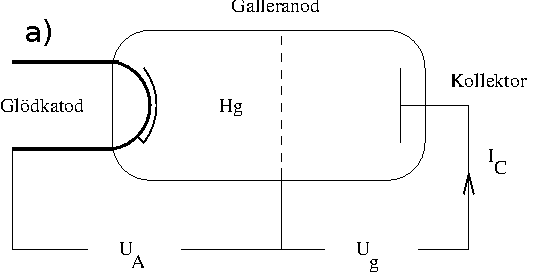
\includegraphics[width=.7\textwidth]{FHtube.png}
	\caption{Frank-Hertz tub.\cite{handledning}}
	\label{fig:tubesch}
\end{figure}

\subsection*{Teori}
En elektrons energi kan bestämmas av dess kinetiska energi. För att kunna exitera en Kvicksilveratom måste denna energi stämma perfekt överrens med exitationsenergin för ett av atomens elektronlager.
Denna lab undersöker vid vilka spänningar vi har toppar och bottnar för att avgöra energin. Denna energi kan beräknas till en våglängd av ljus och på så sätt jämföras mot dess ljusspektra, se \Cref{fig:hgspec}.% och \autoref{fig:hgwl}.

Experimentets utförande är tydligt detaljerat stegvis i handledningen\cite{handledning} och upprepas därför inte här. 
\begin{figure}[hb]
	\centering
	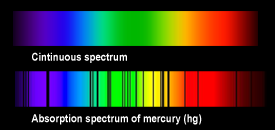
\includegraphics[width=.7\textwidth]{HgSpec.png}
	\caption{Kvicksilver absorbtionsspectrum.\cite{astronoo}}
	\label{fig:hgspec}
\end{figure}

%\begin{figure}[h]
%	\centering
%	\begin{subfigure}[c]{0.63\textwidth}
%	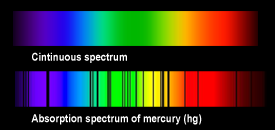
\includegraphics[width=\textwidth]{HgSpec.png}
%	\caption{Kvicksilver absorbtionsspectrum.\cite{astronoo}}
%	\label{fig:hgspec}
%	\end{subfigure}
%	~
%	\begin{subfigure}[c]{0.32\textwidth}
%	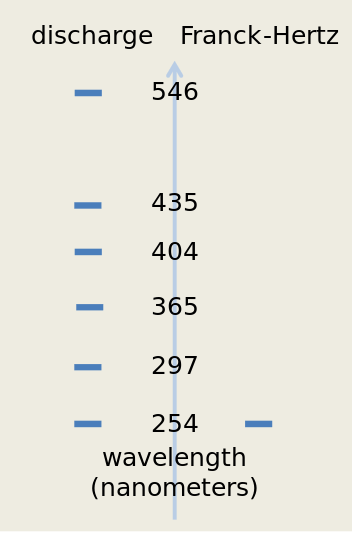
\includegraphics[width=\textwidth]{HgWavelen.png}
%	\caption{Take this picture away.}
%	\label{fig:hgwl}
%	\end{subfigure}
%	\caption{stuff}\label{fig:hgstuff}
%\end{figure}
\newpage

\section{Resultat}
Med ett svep på $50~\textrm{V}$ accelerationsspänning, $U_A$, gavs följande vy, \Cref{fig:ollle} och värdena i \Cref{tab:maxmin}.
\begin{figure}[h]
	\centering
	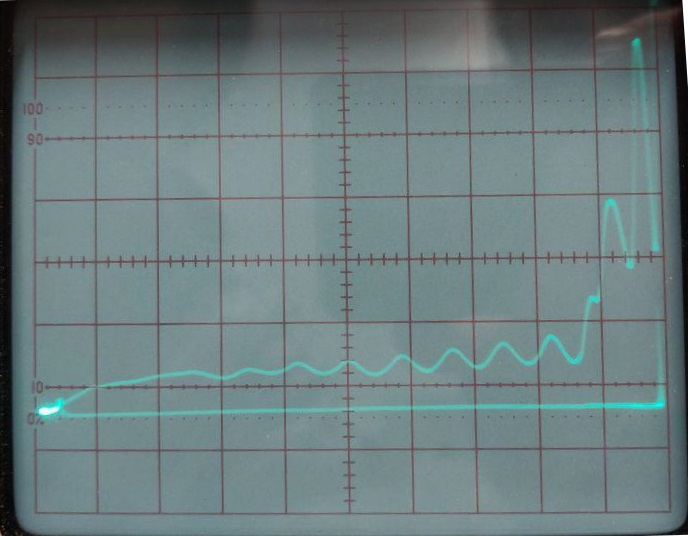
\includegraphics[width = .8\textwidth]{osc_light_low_lowUA_e.jpg}
	\caption{x-led: accelerationsspänning, $U_A$, [$5~\textrm{V/Major div.}$]\\
			y-led: ström, $I_A$, [arbiträr enhet]}
	\label{fig:ollle}
\end{figure}

\begin{minipage}{\linewidth}
\begin{table}[H]
\centering
	\begin{tabular}{llll}
 	\textbf{Maxima [div.]}& \textbf{Maxima [V]}&\textbf{Minima [div.]}& \textbf{Minima [V]}\\\hline
	$3.4$&$17$&$3.0$&15\\
	$4.2$&$21$&$3.8$&19\\
	$5.0$&$25$&$4.6$&23\\
	$5.8$&$29$&$5.4$&27\\
	$6.6$&$33$&$6.2$&31\\
	$7.4$&$37$&$7.0$&35\\
	$8.2$&$41$&$7.8$&39\\
	$8.8$&$44$&$8.4$&42\\
	$9.0$&$45$&$ - $&
 	\end{tabular}
\caption{Maxima och minima i [divisioner] (för jämförelse mot graf) och [V] för analys. Data utläst från graf \cref{fig:ollle}}
\label{tab:maxmin}
\end{table}
\end{minipage}
\vspace{.5cm}

Från \Cref{fig:ollle} kan det ses hur strömmen ökar exponentiellt med högre accelerationsspänning med periodiska dipp som motsvarar excitationsenergierna för kvicksilver. Den exponentiella ökningen ses tydligt i början av \Cref{fig:dark_high} där vi testade extremerna för systemet.

Från jämförelse mellan bilderna \cref{fig:dark_lowub,fig:dark_highub} kan vi se att en skillnad i spänningen över filamentet ``förskjuter'' området vi ser maximan och miniman. 
%Filament voltage effect:
%Scales up or shifts current earlier along the acceleration voltage axis.

\begin{figure}[h]
	\centering
	\begin{subfigure}[c]{0.47\textwidth}
	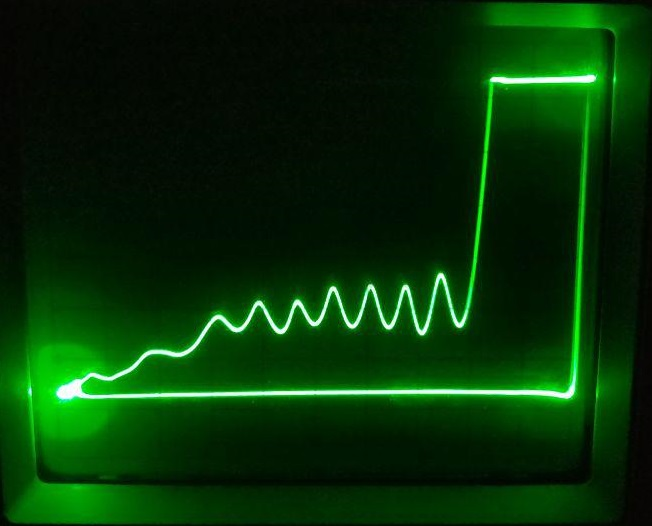
\includegraphics[width=\textwidth]{osc_dark_low_lowUA_e.jpg}
	\caption{XXX}
	\label{fig:dark_lowub}
	\end{subfigure}
	~
	\begin{subfigure}[c]{0.49\textwidth}
	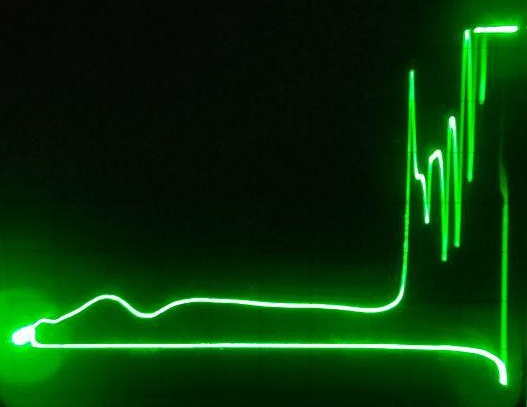
\includegraphics[width=\textwidth]{osc_dark_low_highUA_e.jpg}
	\caption{XXXXXXXXXXX}
	\label{fig:dark_highub}
	\end{subfigure}
	
	\begin{subfigure}[c]{0.47\textwidth}
	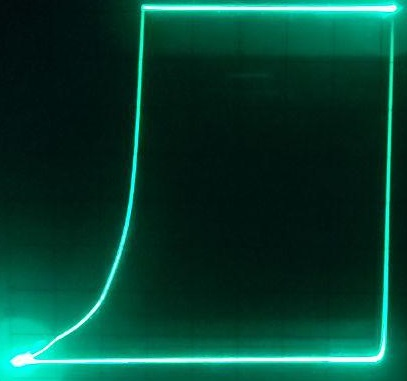
\includegraphics[width=\textwidth]{osc_dark_high_e.jpg}
	\caption{XXXXXXXXXXX}
	\label{fig:dark_high}
	\end{subfigure}
	\caption{XXX}\label{fig:hgstuff}
\end{figure}

%1. description of the experimental setup.
%2. Explain how current, accelerating voltage, reverse bias and collector current should fit
%together if the laws of classical physics would apply.
%3. Using quantum mechanics how would you explain the connection between IC and UA.
%Give an account for the values of accelerating voltages for the different maxima and
%minima, present your results in a table. From these values deduce the excitation energy.
%Take great care in your explanation of the experiment. To facilitate your process of
%understanding you can perform an ’gedanken experiment’ like following an electron as
%it is moving from the source to the collector. Ask yourself questions like, where in
%the tube will excitations occur, what happens to the electron after exciting a mercury
%atom, if an electron of constant kinetic energy (like 1eV) would move from the glowing
%filament to the collector how long would this take, how much is this in comparison to
%the time it takes to complete one cycle (at 50Hz).
%4. In your report you should also include an analysis of what happens to the current
%curve if you change the reverse bias, the current in the glowing filament, the maximum
%acceleration voltage and the temperature of the oven.
\newpage

\section{Diskussion}
Om systemet ses från ett klassiskt mekaniskt perspektiv så består det av en elektron, en partikel, som får en initiell rörelseenergi från accelerationsspänningen, som måste färdas genom ett kontinuerligt retarderande fält i form av kvicksilvergasen och sedan passera potentialsteget som kommer från backspäningen innan den kan bidra till den uppmätta strömmen. 

För en given filamentspänning, kammartemperatur och backspänning kommer partikelflödet öka proportionerligt mot accelerationsspänningen, så den mätta strömmen borde ses som en ramp på oscilloskopet. På grund av backspänningen borde det ses en gräns längs accelerationsspänningsaxeln under vilken ingen ström syns då partiklarna inte har nog energi för att passera barriären. Om filamentspänningen ökas frigörs ett större antal elektroner som kan svepas av accelerationsspänningen, så rampen börjar på samma ställe men blir brantare. Om nu kammartemperaturen ändras så ändras mängden förångat kvicksilver; högre temperatur ger mer kvicksilver som kan absorbera energi från elektronerna. Därför borde temperaturkontrollen ge liknande resultat som backspänningen; senare start på rampen då mer kvicksilver ger större total absorption efter elektronens färd genom molnet.

%Det som faktiskt observerats är BADASS RUBBER DUCKBADASS RUBBER DUCK.

Enligt tabellen \cref{tab:maxmin} har vi miniman i spänningar $15, 19, 23, 27, 31, 35, 39, 42~\textrm{V}$. Då effekten av backspänningen börjar kicka in på slutet observerar vi bara de första $6$ spänningarna. Det kan antas att med rätt justeringar på backspänningen bör detta mönster upprepas både ner till det första kvantstadiet och säkert även för högre spänningar, smartast hade nog varit att zooma in på det tidiga området på plats, men det blev inte av. Ett tydligt mönster på cirka $\Delta 4~\textrm{V/peak}$ kan urskiljas. Denna energi bör stämma överrens med en våglängd av ljus emmiterad av kvicksilver. Användandes \cref{eq:fin} i \cref{sec:met} ges en våglängd på cirka $1.015*10^{-12}~\textrm{m}$, eller $1.015~\textrm{pm}$, se \cref{eq:voltsol}. %Ska vara ~254nm, vet inte varför det är fel, men whatever. Inte fel på formeln jag använt iallafall, den ger samma svar... Tänker nog fel på E_k!
\[\lambda \approx \sqrt{\frac{4.12*10^-24}{V}} = \]
\begin{equation}\label{eq:voltsol} = 1.015*10^{-12}\end{equation}

Detta känns inte riktigt rimligt, men vad gör man?

%3. Using quantum mechanics how would you explain the connection between IC and UA.

%Give an account for the values of accelerating voltages for the different maxima and minima, present your results in a table. From these values deduce the excitation energy.
%Take great care in your explanation of the experiment. To facilitate your process of understanding you can perform an ’gedanken experiment’ like following an electron as it is moving from the source to the collector. Ask yourself questions like, where in the tube will excitations occur, what happens to the electron after exciting a mercury atom, if an electron of constant kinetic energy (like 1eV) would move from the glowing filament to the collector how long would this take, how much is this in comparison to the time it takes to complete one cycle (at 50Hz).


\end{document}
